\documentclass{article}

\usepackage{summary}

\subject{Informationsgestützte Modellierung von Organisationen}
\semester{Summer 2024}
\author{Leopold Lemmermann}

\begin{document}\createtitle

\section{Grundbegriffe}
\begin{figure}
  \centering
  \resizebox{0.5\textwidth}{!}{%
    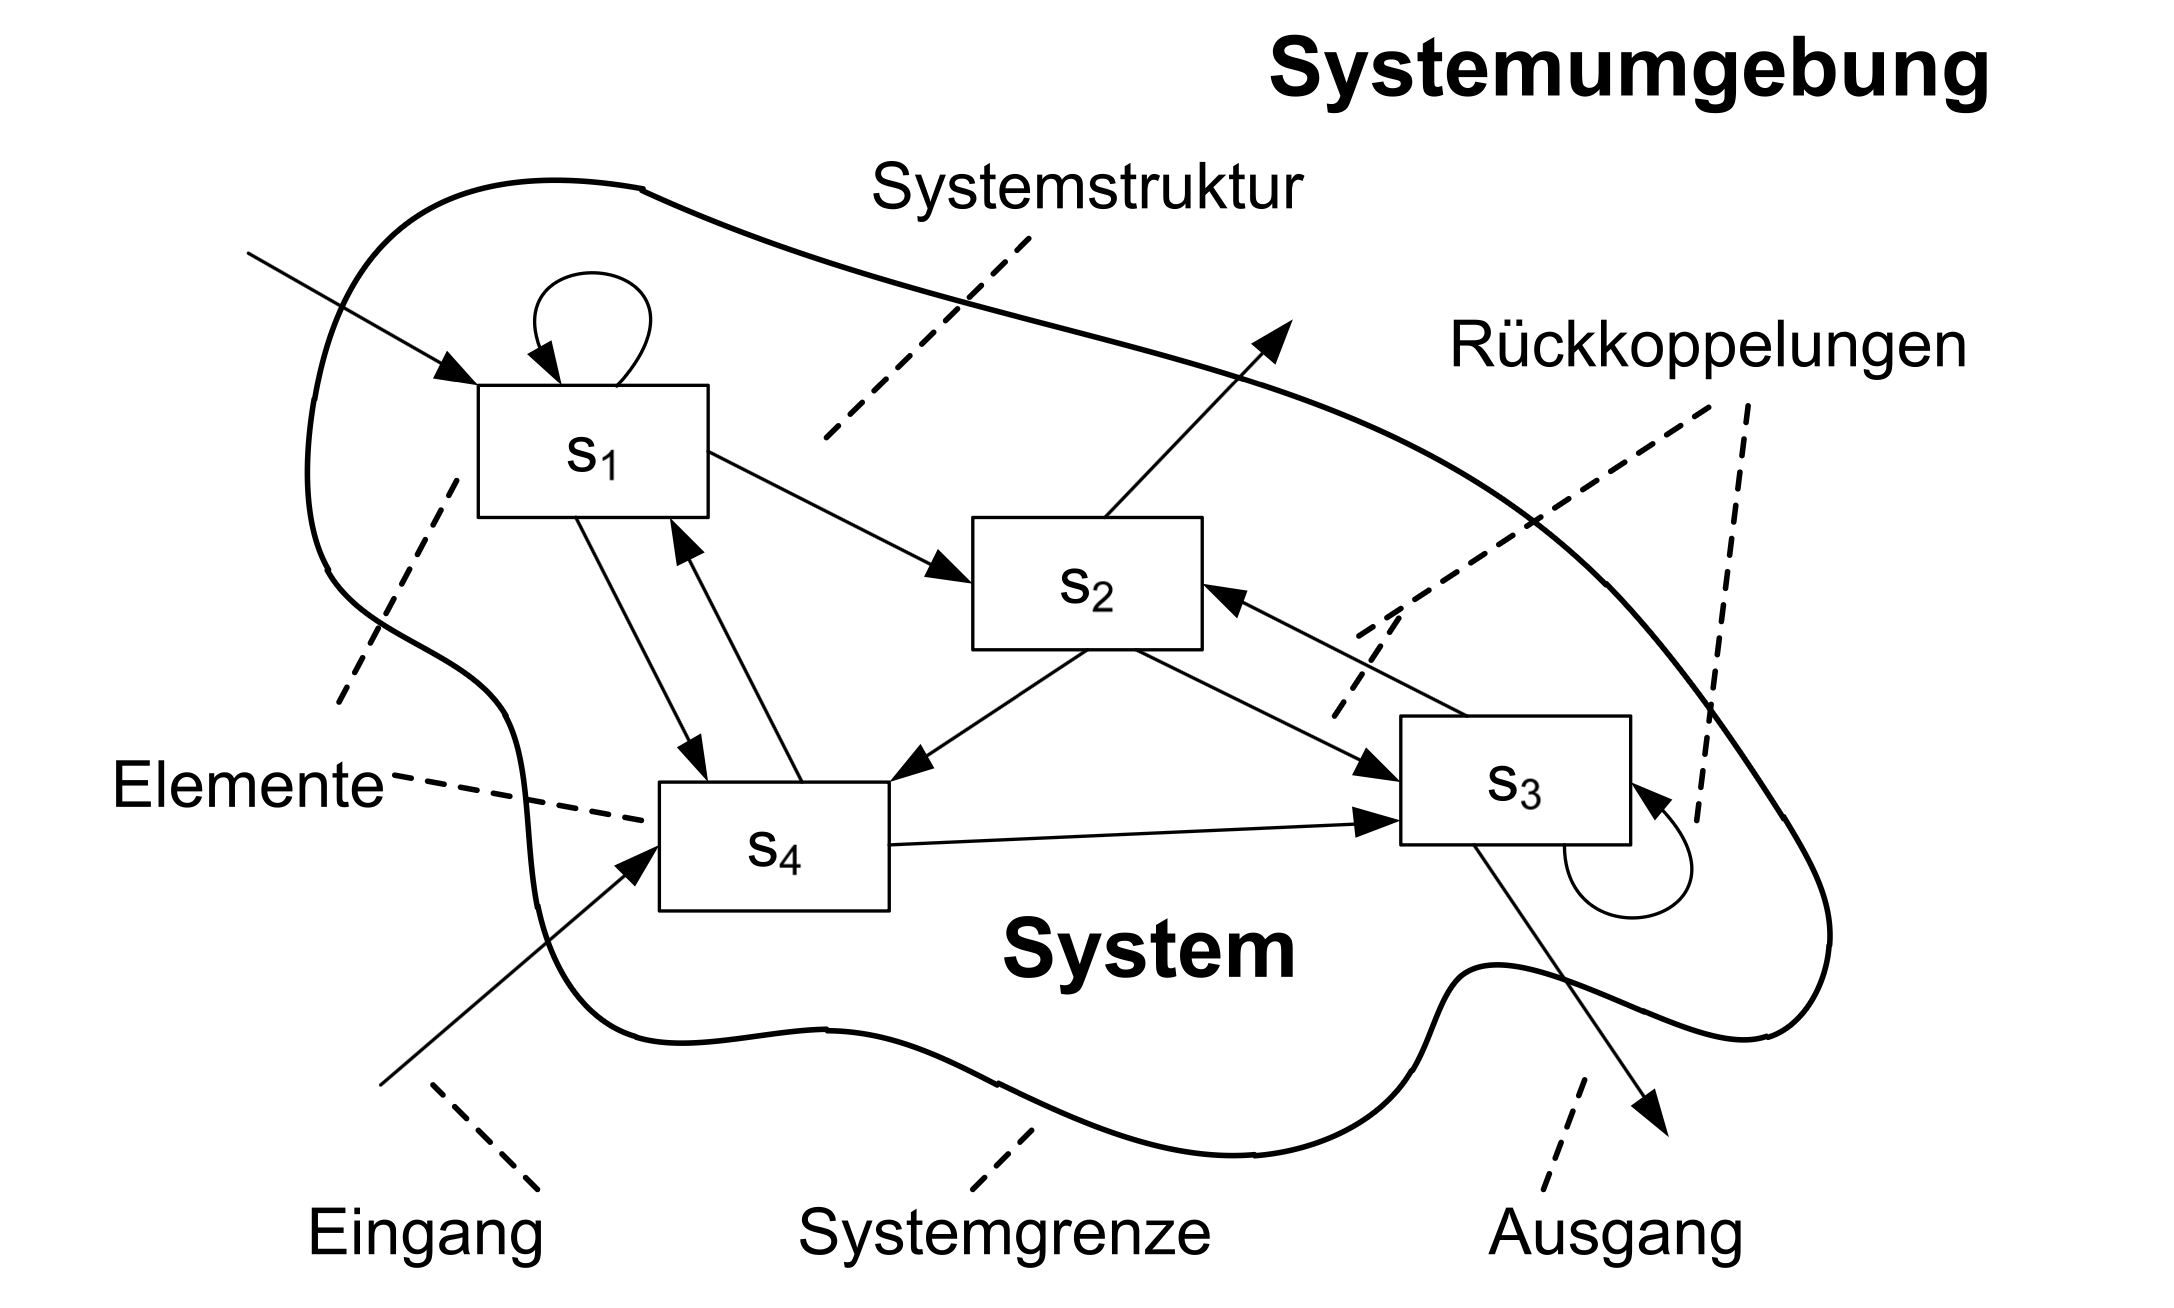
\includegraphics{res/system.png}
  }
  \caption{System}
\end{figure}

\begin{itemize}
  \item \textbf{System}: Ausschnitt aus Gesamtmenge der Objekte \& Beziehunge
  \item \textbf{Systemtheorie}: Erforschung allgemeiner Prinzipien von Systemen
  \item \textbf{Objekt}: (auch Element) kleinste Komponenten eines Systems
  \item \textbf{Zustand}: Menge der Eigenschaften/Zustandsvariablen zu einem Zeitpunkt
  \item \textbf{Verhalten}: dynamische Zustandsfolgen
\end{itemize}

\subsection{Charakteristika}
\begin{itemize}
  \item \textbf{Komplexität}: Anzahl der Elemente, Beziehungen, Zustände
  \item \textbf{Offenheit}: Austausch mit Umwelt
  \item \textbf{Dynamik}: ($\not\leftrightarrow$ Statik) Veränderung über Zeit
  \item \textbf{Kybernetik}: Berücksichtigung von Rückkopplungen
\end{itemize}

\subsection{Modellierung}
\begin{quote}vereinfachende Abbildung (Occam's Razor) eines Systems: \textit{More an art, than a science!}\end{quote}

\begin{itemize}
  \item \textbf{Abstraktion}: Weglassen von Details
  \item \textbf{Idealisierung}: Außerachtlassen von Unerwünschtem \& Irrationalem
\end{itemize}

\subsubsection{Motivationen mit Beispiel}
\begin{itemize}
  \item \textbf{Erklärung}: Stadtplan
  \item \textbf{Prognose}: Wettervorhersage
  \item \textbf{Gestaltung}: Flugzeugdesign
  \item \textbf{Optimierung}: Produktionsplanung
\end{itemize}

\subsection{Simulation}
\begin{quote}Nachahmung von Experimenten an Modellen.\end{quote}

\begin{table}
  \centering
  \begin{tabular}{c|c}
    Vorteile                         & Nachteile \\
    \hline
    \begin{minipage}{0.45\textwidth}
      \begin{itemize}
        \item Realitätsnähe (weniger Annahmen)
        \item unterschiedlicher Detaillierungsgrad
        \item Sensitivity Analysis
        \item mathematisch weniger anspruchsvoll
        \item auch alternative Systemstrukturen
        \item anschaulicher
      \end{itemize}
    \end{minipage} &
    \begin{minipage}{0.45\textwidth}
      \begin{itemize}
        \item Entwicklungsaufwand
        \item Rechenaufwand
        \item Datenbedarf
        \item keine garantierte Optimalität
      \end{itemize}
    \end{minipage}
  \end{tabular}
  \caption{Vor- \& Nachteile gegenüber analytischen Modellen}
\end{table}

\subsubsection{Begrifflichkeiten}
\begin{itemize}
  \item \textbf{Modellierung}: (Modell) Wie funktioniert das System?
  \item \textbf{Simulation}: (Output) Was ist das Ergebnis?
  \item \textbf{Optimierung}: (Input) Wie wird es erreicht?
\end{itemize}

\subsection{Modellbildungszyklus}
\begin{enumerate}
  \item \textbf{Problemdefinition}
  \item \textbf{Entwurf} (+ Datenerhebung): konzeptuelles Modell
  \item \textbf{Implementierung}: Sprache, Werkzeuge, Automatisierung
  \item \textbf{Validierung}: Gültigkeit, Güte
  \item \textbf{Simulation}: statistische Experimentplanung
  \item \textbf{Analyse}: statistisch, Interpretation unter Berücksichtigung von Modelleinschränkungen
  \item \textbf{Dokumentation}: Parallel zu allen Phasen
  \item \textbf{Anwendung}
\end{enumerate}

\subsubsection{Wissenschaft \& Computerspiele}
\begin{table}
  \centering
  \begin{tabular}{r|c|c|c|c|c|c}
    Merkmal      & Daten    & Validierung      & Interaktivität & Zweck        & Software      & Animation   \\
    \hline
    Wissenschaft & real     & zwingend         & selten         & Vorhersage   & spezialisiert & optional    \\
    Spiel        & variiert & faires Spielziel & zwingend       & Unterhaltung & generisch     & sehr häufig \\
  \end{tabular}
  \caption{Vergleich von wissenschaftlichen Modellen \& Computerspielen}
\end{table}
\end{document}